\chapter{Kristal II: Padatan Ion, Kovalen, dan Molekuler}\label{ch:b1:crystals-ionic-covalent}

Garam dapur, jika digerus, pecah menjadi kubus-kubus kecil; intan adalah
bahan alam yang paling keras, tetapi grafit, yang tersusun atas atom
karbon yang sama, cukup lunak untuk dipakai menulis; es mengapung di atas
air. Semuanya \omterm{def:b1:crystals-metals:crystal}{kristal}, tetapi partikel-partikelnya diikat dengan cara
yang berbeda: ion oleh tarikan elektrostatik, atom oleh \omterm{def:b1:lewis-resonance-vsepr:lewis}{ikatan kovalen},
molekul oleh gaya-gaya antarmolekul pada
\cref{ch:b1:intermolecular-forces-solvents}. Bab ini menerapkan geometri
sel dari bab sebelumnya pada ketiga golongan padatan ini, dan menjelaskan,
dari ukuran ion-ionnya, mengapa natrium klorida dan sesium klorida
mengambil struktur yang berbeda.

\begin{recall}
\omterm{def:b1:crystals-metals:multiplicity}{Multiplisitas}, \omterm{def:b1:crystals-metals:coordination}{bilangan koordinasi}, dan \omterm{def:b1:crystals-metals:compactness}{kekompakan} sebuah sel, serta
situs-situs oktahedral dan tetrahedral \omterm{def:b1:crystals-metals:lattice}{kisi} \omterm{def:b1:crystals-metals:packings}{kubus berpusat muka},
didefinisikan pada \cref{ch:b1:crystals-metals}; massa jenis sebuah
\omterm{def:b1:crystals-metals:crystal}{kristal} adalah $\rho = ZM/(N_A V)$
(\cref{prop:b1:crystals-metals:density}). \omterm{def:b1:periodicity:radius}{Jari-jari ion} diperkenalkan
pada \cref{def:b1:periodicity:radius}.
\end{recall}

\section{Kristal ion dan rasio jari-jari}

\begin{definition}[Kristal ion]\label{def:b1:crystals-ionic-covalent:ionic-crystal}
\emph{Kristal ion}\index{kristal ion} adalah \omterm{def:b1:crystals-metals:crystal}{kristal} yang tersusun atas
kation dan anion yang diikat oleh tarikan elektrostatik. Setiap ion
dikelilingi ion-ion yang muatannya berlawanan; \omterm{def:b1:crystals-metals:crystal}{kristal} itu netral secara
listrik, sehingga banyaknya kation dan anion dalam sebuah sel berbanding
sesuai rumusnya.
\end{definition}

\begin{proposition}[Sifat-sifat kristal ion]\label{prop:b1:crystals-ionic-covalent:ionic-properties}
\omterm{def:b1:crystals-ionic-covalent:ionic-crystal}{Kristal ion} keras tetapi rapuh (pergeseran satu lapisan menghadapkan
ion-ion yang muatannya sejenis, dan \omterm{def:b1:crystals-metals:crystal}{kristal} itu terbelah), titik lelehnya
tinggi, tidak menghantarkan listrik dalam keadaan padat tetapi
menghantarkannya dalam keadaan lebur atau terlarut, dan larut dalam
\omterm{def:b1:intermolecular-forces-solvents:solvent-classes}{pelarut polar} yang permitivitasnya tinggi.
\end{proposition}
\admitted

\begin{definition}[Rasio jari-jari]\label{def:b1:crystals-ionic-covalent:radius-ratio}
Dalam \omterm{def:b1:crystals-ionic-covalent:ionic-crystal}{kristal ion} yang tersusun atas kation berjari-jari $r_+$ dan anion
berjari-jari $r_-$, \emph{rasio jari-jari}\index{rasio jari-jari} adalah
$x = r_+/r_-$ (biasanya $x < 1$, karena kation lebih kecil daripada
anion).
\end{definition}

\begin{proposition}[Aturan rasio jari-jari]\label{prop:b1:crystals-ionic-covalent:rule}
Dalam model bola keras, struktur yang setiap kationnya menyentuh $n$
anion hanya stabil jika anion-anion tidak saling bersentuhan, yang
menuntut $x$ di atas suatu batas yang ditentukan oleh geometrinya:
$x \ge \sqrt3 - 1
\approx 0.732$ untuk 8 tetangga (kubus), $x \ge \sqrt2 - 1 \approx 0.414$
untuk 6 (oktahedron), $x \ge \sqrt{3/2} - 1 \approx 0.225$ untuk 4
(tetrahedron). Struktur yang diambil adalah struktur dengan koordinasi
tertinggi yang diizinkan oleh $x$.
\end{proposition}

\begin{proof}
Kation duduk di dalam celah di antara $n$ anion yang menyentuhnya. Pada
batasnya, anion-anion juga saling bersentuhan. Kubus: anion-anion berada
di sudut-sudut kubus berusuk $2r_-$ dan kation di pusatnya, sehingga $r_+ +
r_- = \sqrt3\,r_-$. Oktahedron: empat anion pada sebuah bujur sangkar
bersisi $2r_-$, kation di pusatnya, $r_+ + r_- = \sqrt2\,r_-$.
Tetrahedron: anion-anion di sudut-sudut yang berselang-seling pada kubus
berusuk $\sqrt2\,r_-$, kation di pusatnya,
$r_+ + r_- = \frac{\sqrt3}{2}\sqrt2\,r_- = \sqrt{3/2}\,r_-$.
Dengan membaginya dengan $r_-$ diperoleh batas-batas itu. Di bawah batas,
kation berguncang di dalam celah yang terlalu besar baginya: anion-anion
saling tolak tanpa tarikannya bertambah, sehingga koordinasi yang lebih
rendah, dengan celah yang lebih kecil, lebih disukai.
\end{proof}

\begin{omfigure}
\begin{tikzpicture}[font=\small, >={Stealth}]
  \draw[->, thick] (0,0) -- (12.4,0) node[right] {$x = r_+/r_-$};
  \foreach \x/\l in {0/0, 2.7/0.225, 4.97/0.414, 8.78/0.732, 12/1} {
    \draw (\x,0.12) -- (\x,-0.12) node[below] {\l};
  }
  \fill[omDef!15] (2.7,0.2) rectangle (4.97,1.0);
  \fill[omProp!15] (4.97,0.2) rectangle (8.78,1.0);
  \fill[omThm!15] (8.78,0.2) rectangle (12,1.0);
  \node[align=center] at (3.83,0.6) {4: ZnS};
  \node[align=center] at (6.87,0.6) {6: NaCl};
  \node[align=center] at (10.4,0.6) {8: CsCl};
  \foreach \x/\l in {3.91/\ce{ZnS}, 6.76/\ce{NaCl}, 10.08/\ce{RbCl}, 11.54/\ce{CsCl}} {
    \draw[omExo, thick] (\x,-0.55) -- (\x,-0.95);
    \node[below, omExo] at (\x,-0.95) {\l};
  }
\end{tikzpicture}

{\small Aturan \omterm{def:b1:crystals-ionic-covalent:radius-ratio}{rasio jari-jari}: \omterm{def:b1:crystals-metals:coordination}{bilangan koordinasi} kation yang diizinkan
oleh $x$, dan rasio terukur empat garam (jari-jari Shannon). Rubidium
klorida, pada 0.84, semestinya bertipe \ce{CsCl}, tetapi mengambil tipe
\ce{NaCl}: aturan itu pedoman, bukan hukum
(\cref{exo:b1:crystals-ionic-covalent:12}).}
% ledger: rion:Zn2+IV, rion:S2-VI, rion:Na+VI, rion:Cl-VI, rion:Rb+VI,
% rion:Cs+VIII
\end{omfigure}

\section{Empat tipe struktur}

\begin{definition}[Tipe struktur]\label{def:b1:crystals-ionic-covalent:structure-type}
\omterm{def:b1:crystals-ionic-covalent:ionic-crystal}{Kristal ion} digolongkan menurut beberapa tipe struktur, yang dinamai
menurut sebuah senyawa wakilnya:
\begin{itemize}
  \item \emph{tipe sesium klorida}\index{tipe sesium klorida}: anion di
        sudut-sudut kubus, kation di pusatnya (8:8);
  \item \emph{tipe garam batu}\index{tipe garam batu} (tipe natrium
        klorida): anion pada \omterm{def:b1:crystals-metals:lattice}{kisi} FCC, kation di semua \omterm{def:b1:crystals-metals:site}{situs
        oktahedralnya} (6:6);
  \item \emph{tipe sfalerit}\index{tipe sfalerit} (seng blende): anion
        pada \omterm{def:b1:crystals-metals:lattice}{kisi} FCC, kation di separuh \omterm{def:b1:crystals-metals:site}{situs tetrahedralnya}, satu dari
        dua secara berselang-seling (4:4);
  \item \emph{tipe fluorit}\index{tipe fluorit}: kation pada \omterm{def:b1:crystals-metals:lattice}{kisi} FCC,
        anion di semua \omterm{def:b1:crystals-metals:site}{situs tetrahedralnya} (8:4), rumus \ce{MX2}; pada
        \emph{tipe antifluorit}\index{tipe antifluorit} peran keduanya
        dipertukarkan (\ce{Li2O}, 4:8).
\end{itemize}
Pasangan bilangan itu menyatakan koordinasi kation dan koordinasi
anion.
\end{definition}

\begin{omfigure}
\tdplotsetmaincoords{60}{100}
\begin{tikzpicture}[tdplot_main_coords, font=\small]
  \pic {omcubeo={3}};
    \node[aX={green!55!black}{6.5mm}] at (0,0,0) {};
  \node[aX={violet!70}{3.8mm}] at (0,1.5,0) {};
  \node[aX={green!55!black}{6.5mm}] at (0,3,0) {};
  \node[aX={violet!70}{3.8mm}] at (0,0,1.5) {};
  \node[aX={green!55!black}{6.5mm}] at (0,1.5,1.5) {};
  \node[aX={violet!70}{3.8mm}] at (0,3,1.5) {};
  \node[aX={violet!70}{3.8mm}] at (1.5,0,0) {};
  \node[aX={green!55!black}{6.5mm}] at (0,0,3) {};
  \node[aX={green!55!black}{6.5mm}] at (1.5,1.5,0) {};
  \node[aX={violet!70}{3.8mm}] at (0,1.5,3) {};
  \node[aX={violet!70}{3.8mm}] at (1.5,3,0) {};
  \node[aX={green!55!black}{6.5mm}] at (0,3,3) {};
  \node[aX={green!55!black}{6.5mm}] at (1.5,0,1.5) {};
  \node[aX={violet!70}{3.8mm}] at (1.5,1.5,1.5) {};
  \node[aX={green!55!black}{6.5mm}] at (1.5,3,1.5) {};
  \node[aX={green!55!black}{6.5mm}] at (3,0,0) {};
  \node[aX={violet!70}{3.8mm}] at (1.5,0,3) {};
  \node[aX={violet!70}{3.8mm}] at (3,1.5,0) {};
  \node[aX={green!55!black}{6.5mm}] at (1.5,1.5,3) {};
  \node[aX={green!55!black}{6.5mm}] at (3,3,0) {};
  \node[aX={violet!70}{3.8mm}] at (1.5,3,3) {};
  \node[aX={violet!70}{3.8mm}] at (3,0,1.5) {};
  \node[aX={green!55!black}{6.5mm}] at (3,1.5,1.5) {};
  \node[aX={violet!70}{3.8mm}] at (3,3,1.5) {};
  \node[aX={green!55!black}{6.5mm}] at (3,0,3) {};
  \node[aX={violet!70}{3.8mm}] at (3,1.5,3) {};
  \node[aX={green!55!black}{6.5mm}] at (3,3,3) {};
  \node at (1.5,1.5,-1.75) {\ce{NaCl} (garam batu)};
\end{tikzpicture}
\hspace{1cm}
\begin{tikzpicture}[tdplot_main_coords, font=\small]
  \pic {omcubeo={3}};
    \node[aX={green!55!black}{6.5mm}] at (0,0,0) {};
  \node[aX={green!55!black}{6.5mm}] at (0,3,0) {};
  \node[aX={green!55!black}{6.5mm}] at (0,0,3) {};
  \node[aX={green!55!black}{6.5mm}] at (0,3,3) {};
  \node[aX={blue!60}{7mm}] at (1.5,1.5,1.5) {};
  \node[aX={green!55!black}{6.5mm}] at (3,0,0) {};
  \node[aX={green!55!black}{6.5mm}] at (3,3,0) {};
  \node[aX={green!55!black}{6.5mm}] at (3,0,3) {};
  \node[aX={green!55!black}{6.5mm}] at (3,3,3) {};
  \node at (1.5,1.5,-1.75) {\ce{CsCl}};
\end{tikzpicture}

{\small Kiri: sel garam batu, \ce{Cl-} (hijau) pada \omterm{def:b1:crystals-metals:lattice}{kisi} FCC, \ce{Na+}
(ungu) di setiap \omterm{def:b1:crystals-metals:site}{situs oktahedral}. Kanan: sel sesium klorida, \ce{Cl-} di
sudut-sudut, \ce{Cs+} (biru) di pusat. Ion-ion digambar lebih kecil
daripada ukuran sentuhnya.}
\end{omfigure}

\begin{proposition}[Tipe garam batu dan tipe sesium klorida]\label{prop:b1:crystals-ionic-covalent:nacl-cscl}
Pada \omterm{def:b1:crystals-ionic-covalent:structure-type}{tipe garam batu}, $Z = 4$ satuan rumus per sel, ion-ion bersentuhan
sepanjang rusuk, $a = 2(r_+ + r_-)$, dan struktur itu menuntut
$\sqrt2 - 1
\le x$. Pada \omterm{def:b1:crystals-ionic-covalent:structure-type}{tipe sesium klorida}, $Z = 1$, ion-ion
bersentuhan sepanjang diagonal ruang, $a\sqrt3 = 2(r_+ + r_-)$, dan
struktur itu menuntut $x \ge \sqrt3 - 1$.
\end{proposition}

\begin{proof}
Garam batu: anion-anion \omterm{def:b1:crystals-metals:lattice}{kisi} FCC berjumlah $4$, kation-kation di 4 \omterm{def:b1:crystals-metals:site}{situs
oktahedral} $1 + 12 \times \frac14 = 4$. Sepanjang rusuk, anion, kation,
dan anion berurutan saling bersentuhan. Anion-anion tidak bertumpang
tindih jika diagonal muka, yang memuat tiga anion dengan paling banyak
dua yang bersentuhan, memenuhi $a\sqrt2 \ge 4r_-$, yaitu
$2(r_+ + r_-)\sqrt2 \ge
4r_-$, atau $x \ge \sqrt2 - 1$. Sesium klorida:
$8 \times \frac18 = 1$ anion dan 1 kation; pada diagonal ruang, anion,
kation, anion bersentuhan; anion-anion tidak bertumpang tindih
sepanjang rusuk jika $a \ge 2r_-$, yaitu $2(r_+ + r_-)/\sqrt3 \ge 2r_-$,
atau $x \ge \sqrt3 - 1$.
\end{proof}

\begin{example}[Natrium klorida dan sesium klorida]\label{ex:b1:crystals-ionic-covalent:nacl}
Natrium klorida mempunyai $a = \qty{564.1}{pm}$: $r_+ + r_- = a/2 =
\qty{282.0}{pm}$, dibandingkan dengan $102 + 181 = \qty{283}{pm}$ dari
jari-jari Shannon; $x = 102/181 = 0.56$, dalam rentang oktahedral.
Massa jenisnya $\rho = 4 \times 58.44/(6.022 \times 10^{23} \times (5.641 \times
10^{-8})^3) = \qty{2.16}{g/cm^3}$, terukur \qty{2.17}{g/cm^3}. Sesium
klorida mempunyai $a = \qty{412.3}{pm}$: $r_+ + r_- = a\sqrt3/2 =
\qty{357.1}{pm}$, dan $x = 174/181 = 0.96$, dalam rentang kubus.
% ledger: lat:NaCl, rion:Na+VI, rion:Cl-VI, rho:NaCl, lat:CsCl,
% rion:Cs+VIII
\end{example}

\begin{omfigure}
\begin{minipage}[b]{0.31\linewidth}\centering
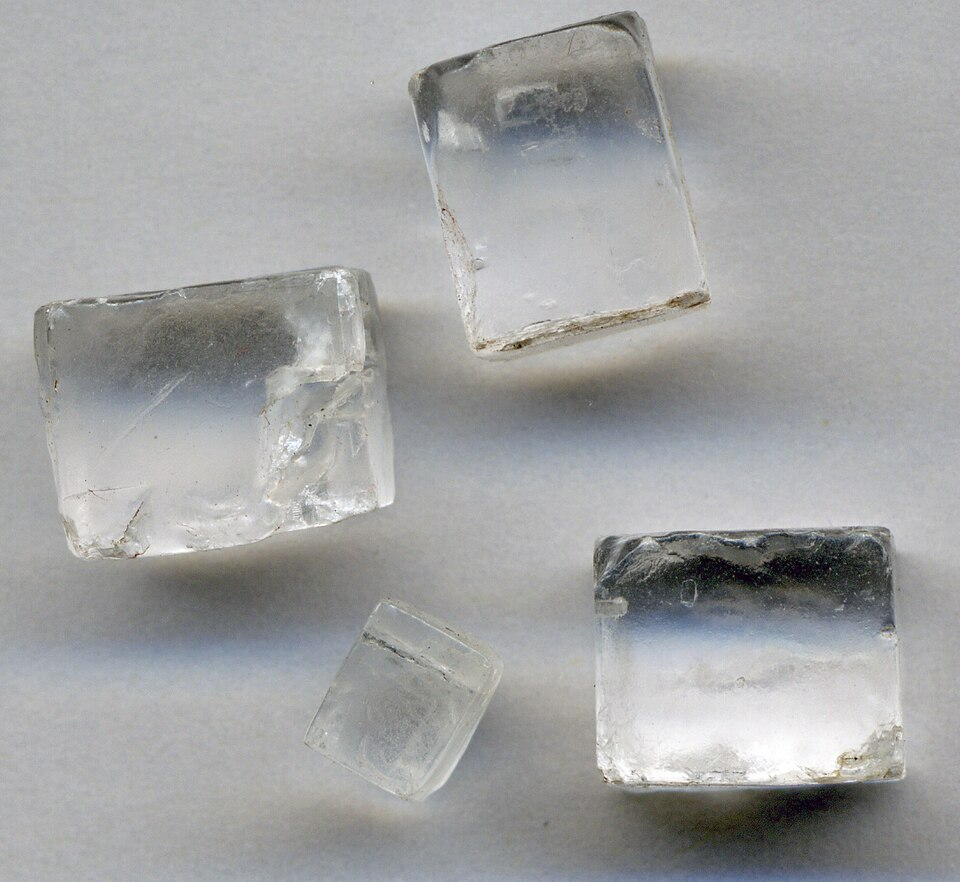
\includegraphics[width=\linewidth]{images/book2/halite.jpg}

{\small \omterm{def:b1:crystals-metals:crystal}{Kristal} halit (garam batu). Foto: James St. John, CC BY 2.0.}
\end{minipage}\hfill
\begin{minipage}[b]{0.31\linewidth}\centering
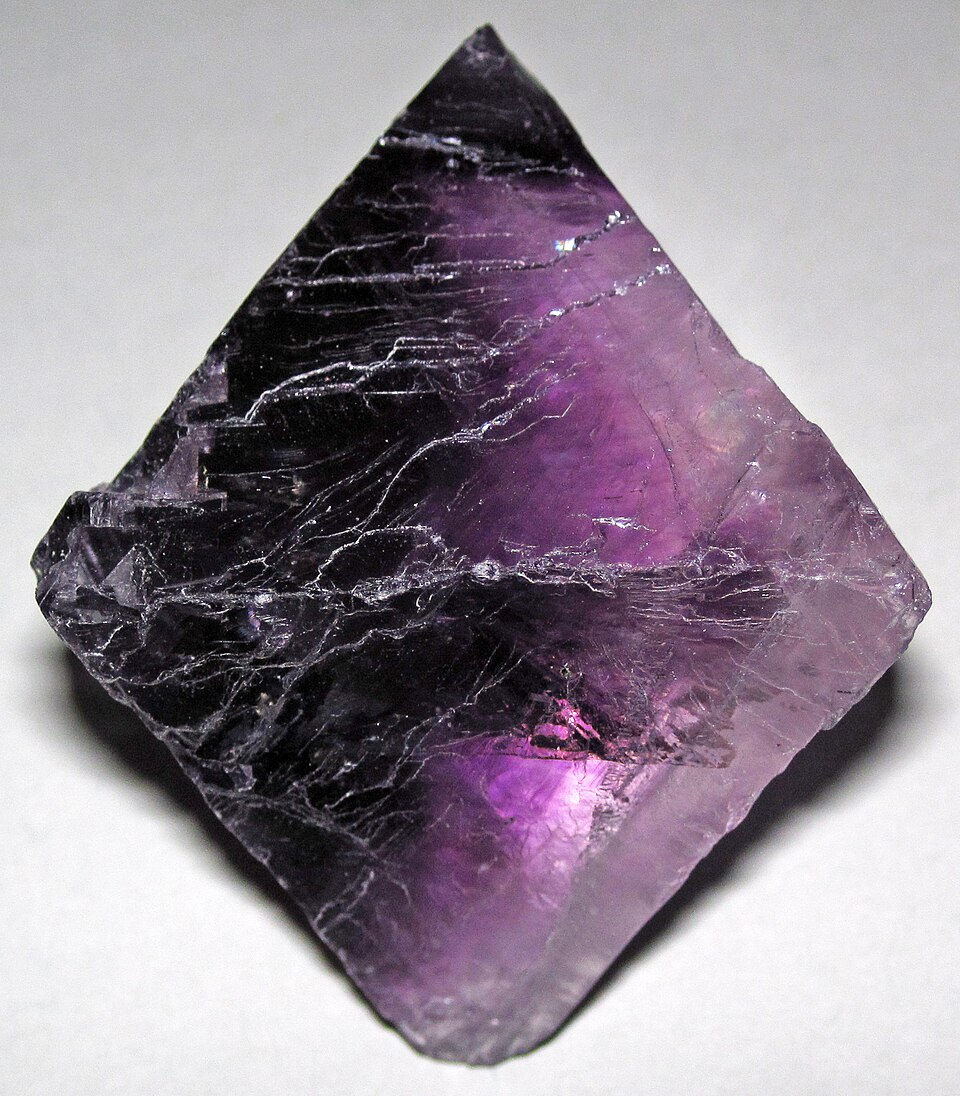
\includegraphics[width=0.85\linewidth]{images/book2/fluorite.jpg}

{\small Fluorit, \ce{CaF2}. Foto: James St. John, CC BY 2.0.}
\end{minipage}\hfill
\begin{minipage}[b]{0.31\linewidth}\centering
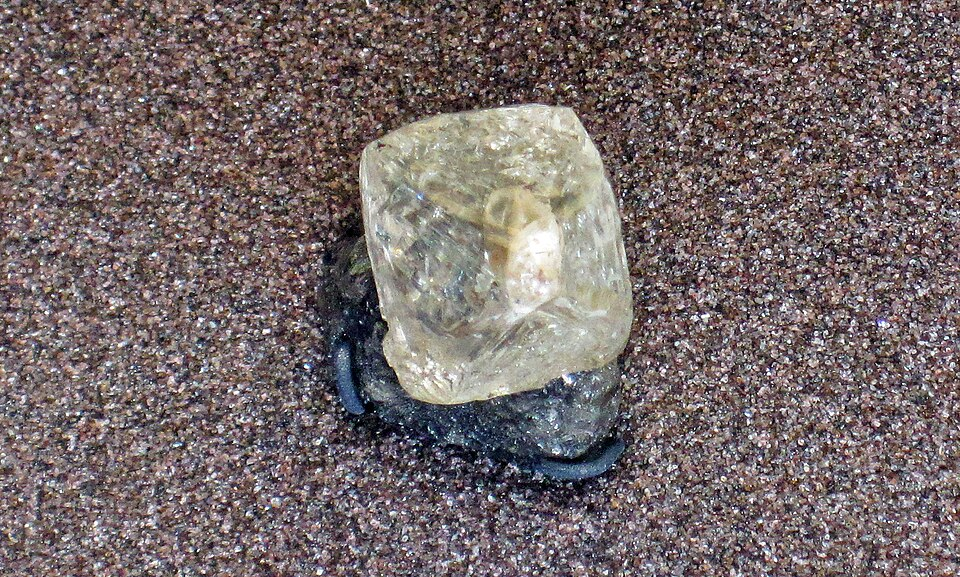
\includegraphics[width=\linewidth]{images/book2/diamond.jpg}

{\small Oktahedron intan kasar. Foto: James St. John, CC BY 2.0.}
\end{minipage}
\end{omfigure}

\begin{proposition}[Tipe sfalerit dan tipe fluorit]\label{prop:b1:crystals-ionic-covalent:zns-caf2}
Pada \omterm{def:b1:crystals-ionic-covalent:structure-type}{tipe sfalerit}, $Z = 4$, setiap ion dikelilingi empat ion jenis lain
di sudut-sudut sebuah tetrahedron, dan ion-ion bersentuhan sepanjang
seperempat diagonal ruang: $a\sqrt3/4 = r_+ + r_-$. Pada \omterm{def:b1:crystals-ionic-covalent:structure-type}{tipe fluorit},
$Z = 4$ satuan \ce{CaF2}, setiap kation mempunyai 8 tetangga anion
(sebuah kubus), setiap anion 4 tetangga kation (sebuah tetrahedron), dan
sekali lagi $a\sqrt3/4 =
r_+ + r_-$.
\end{proposition}

\begin{proof}
Sfalerit: 4 anion pada \omterm{def:b1:crystals-metals:lattice}{kisi} FCC dan 4 kation di separuh dari 8 \omterm{def:b1:crystals-metals:site}{situs
tetrahedral}. \omterm{def:b1:crystals-metals:site}{Situs tetrahedral} di $(\frac a4,\frac a4,\frac a4)$
berjarak $\frac{a\sqrt3}{4}$ dari keempat anionnya. Fluorit: 4 kation
dan 8 anion di semua \omterm{def:b1:crystals-metals:site}{situs tetrahedral}, rasio $1:2$. Kedelapan anion di
dalam sel membentuk kubus berusuk $a/2$, yang kubus-kubus anionnya
memuat sebuah kation di pusat setiap kubus kedua; sebuah anion mempunyai
4 tetangga kationnya pada jarak $\frac{a\sqrt3}{4}$.
\end{proof}

\begin{omfigure}
\tdplotsetmaincoords{60}{100}
\begin{tikzpicture}[tdplot_main_coords, font=\small]
  \pic {omcubeo={3}};
  \begin{scope}[on background layer]
    \draw[black!45, line width=1.2pt] (0.75,0.75,2.25) -- (0,0,3) (0.75,0.75,2.25) -- (0,1.5,1.5) (0.75,0.75,2.25) -- (1.5,0,1.5) (0.75,0.75,2.25) -- (1.5,1.5,3) (0.75,2.25,0.75) -- (0,1.5,1.5) (0.75,2.25,0.75) -- (0,3,0) (0.75,2.25,0.75) -- (1.5,1.5,0) (0.75,2.25,0.75) -- (1.5,3,1.5) (2.25,0.75,0.75) -- (1.5,0,1.5) (2.25,0.75,0.75) -- (1.5,1.5,0) (2.25,0.75,0.75) -- (3,0,0) (2.25,0.75,0.75) -- (3,1.5,1.5) (2.25,2.25,2.25) -- (1.5,1.5,3) (2.25,2.25,2.25) -- (1.5,3,1.5) (2.25,2.25,2.25) -- (3,1.5,1.5) (2.25,2.25,2.25) -- (3,3,3);
  \end{scope}
    \node[aX={yellow!75!orange}{6mm}] at (0,0,0) {};
  \node[aX={yellow!75!orange}{6mm}] at (0,3,0) {};
  \node[aX={yellow!75!orange}{6mm}] at (0,1.5,1.5) {};
  \node[aX={gray!60}{3.6mm}] at (0.75,2.25,0.75) {};
  \node[aX={yellow!75!orange}{6mm}] at (0,0,3) {};
  \node[aX={yellow!75!orange}{6mm}] at (1.5,1.5,0) {};
  \node[aX={gray!60}{3.6mm}] at (0.75,0.75,2.25) {};
  \node[aX={yellow!75!orange}{6mm}] at (0,3,3) {};
  \node[aX={yellow!75!orange}{6mm}] at (1.5,0,1.5) {};
  \node[aX={gray!60}{3.6mm}] at (2.25,0.75,0.75) {};
  \node[aX={yellow!75!orange}{6mm}] at (1.5,3,1.5) {};
  \node[aX={yellow!75!orange}{6mm}] at (3,0,0) {};
  \node[aX={yellow!75!orange}{6mm}] at (1.5,1.5,3) {};
  \node[aX={yellow!75!orange}{6mm}] at (3,3,0) {};
  \node[aX={gray!60}{3.6mm}] at (2.25,2.25,2.25) {};
  \node[aX={yellow!75!orange}{6mm}] at (3,1.5,1.5) {};
  \node[aX={yellow!75!orange}{6mm}] at (3,0,3) {};
  \node[aX={yellow!75!orange}{6mm}] at (3,3,3) {};
  \node at (1.5,1.5,-1.75) {\ce{ZnS} (sfalerit)};
\end{tikzpicture}
\hspace{1cm}
\begin{tikzpicture}[tdplot_main_coords, font=\small]
  \pic {omcubeo={3}};
    \node[aX={green!35!gray}{4.4mm}] at (0,0,0) {};
  \node[aX={green!35!gray}{4.4mm}] at (0,3,0) {};
  \node[aX={green!35!gray}{4.4mm}] at (0,1.5,1.5) {};
  \node[aX={green!45!yellow}{5.0mm}] at (0.75,0.75,0.75) {};
  \node[aX={green!45!yellow}{5.0mm}] at (0.75,2.25,0.75) {};
  \node[aX={green!35!gray}{4.4mm}] at (0,0,3) {};
  \node[aX={green!35!gray}{4.4mm}] at (1.5,1.5,0) {};
  \node[aX={green!45!yellow}{5.0mm}] at (0.75,0.75,2.25) {};
  \node[aX={green!35!gray}{4.4mm}] at (0,3,3) {};
  \node[aX={green!35!gray}{4.4mm}] at (1.5,0,1.5) {};
  \node[aX={green!45!yellow}{5.0mm}] at (0.75,2.25,2.25) {};
  \node[aX={green!45!yellow}{5.0mm}] at (2.25,0.75,0.75) {};
  \node[aX={green!35!gray}{4.4mm}] at (1.5,3,1.5) {};
  \node[aX={green!35!gray}{4.4mm}] at (3,0,0) {};
  \node[aX={green!45!yellow}{5.0mm}] at (2.25,2.25,0.75) {};
  \node[aX={green!35!gray}{4.4mm}] at (1.5,1.5,3) {};
  \node[aX={green!35!gray}{4.4mm}] at (3,3,0) {};
  \node[aX={green!45!yellow}{5.0mm}] at (2.25,0.75,2.25) {};
  \node[aX={green!45!yellow}{5.0mm}] at (2.25,2.25,2.25) {};
  \node[aX={green!35!gray}{4.4mm}] at (3,1.5,1.5) {};
  \node[aX={green!35!gray}{4.4mm}] at (3,0,3) {};
  \node[aX={green!35!gray}{4.4mm}] at (3,3,3) {};
  \node at (1.5,1.5,-1.75) {\ce{CaF2} (fluorit)};
\end{tikzpicture}

{\small Kiri: sfalerit, \ce{S^{2-}} (kuning) pada \omterm{def:b1:crystals-metals:lattice}{kisi} FCC dan
\ce{Zn^{2+}} (abu-abu) di situs-situs tetrahedral yang berselang-seling,
masing-masing terhubung dengan keempat tetangganya. Kanan: fluorit,
\ce{Ca^{2+}} (hijau keabu-abuan) pada \omterm{def:b1:crystals-metals:lattice}{kisi} FCC dan \ce{F-} (hijau muda)
di kedelapan \omterm{def:b1:crystals-metals:site}{situs tetrahedral}.}
\end{omfigure}

\begin{example}[Sfalerit dan fluorit]\label{ex:b1:crystals-ionic-covalent:zns}
Sfalerit mempunyai $a = \qty{540.9}{pm}$: $r_+ + r_- = a\sqrt3/4 =
\qty{234.2}{pm}$ (Shannon: $60 + 184 = \qty{244}{pm}$, karena jari-jari
sulfida hanya ditabelkan untuk enam tetangga), dan $x = 60/184 = 0.33$,
dalam rentang tetrahedral. Fluorit mempunyai $a = \qty{546.3}{pm}$:
$r_+ + r_- =
\qty{236.6}{pm}$ (Shannon $112 + 131 = \qty{243}{pm}$), dan
$x = 0.85$: kation duduk di dalam kubus yang dibentuk 8 anion, sesuai
tuntutan aturan itu.
% ledger: lat:ZnS, rion:Zn2+IV, rion:S2-VI, lat:CaF2, rion:Ca2+VIII,
% rion:F-IV
\end{example}

\begin{method}[Meramalkan struktur]\label{met:b1:crystals-ionic-covalent:predict}
Untuk meramalkan struktur senyawa ion \ce{MX} atau \ce{MX2}:
\begin{enumerate}
  \item hitunglah $x = r_+/r_-$ dari jari-jari dalam tabel (untuk
        koordinasi yang diharapkan);
  \item bacalah koordinasi kation dari aturan \omterm{def:b1:crystals-ionic-covalent:radius-ratio}{rasio jari-jari};
  \item pilihlah tipe yang mempunyai koordinasi ini dan rumus yang
        tepat: \ce{MX} dengan 8: \ce{CsCl}; dengan 6: \ce{NaCl}; dengan 4:
        sfalerit; \ce{MX2} dengan 8: fluorit;
  \item periksalah dengan \omterm{def:b1:crystals-metals:lattice}{parameter kisi} terukur; ingatlah bahwa ion
        yang mudah terpolarisasi (\ce{S^{2-}}, \ce{I-}) dan kation kecil
        yang bermuatan menghasilkan ikatan yang sebagian kovalen, yang
        membuat aturan itu gagal.
\end{enumerate}
\end{method}

\section{Kristal kovalen}

\begin{definition}[Kristal kovalen]\label{def:b1:crystals-ionic-covalent:covalent-crystal}
\emph{Kristal kovalen}\index{kristal kovalen} (atau padatan jaringan)
adalah \omterm{def:b1:crystals-metals:crystal}{kristal} yang semua atomnya terhubung oleh \omterm{def:b1:lewis-resonance-vsepr:lewis}{ikatan kovalen} menjadi
satu molekul raksasa: intan, silikon, kuarsa \ce{SiO2}. Pada \omterm{def:b1:crystals-metals:crystal}{kristal}
kovalen berlapis seperti grafit, jaringan kovalennya hanya meluas pada
bidang-bidang, yang satu sama lain diikat oleh \omterm{def:b1:intermolecular-forces-solvents:vdw}{interaksi van der Waals}.
\end{definition}

\begin{proposition}[Struktur intan]\label{prop:b1:crystals-ionic-covalent:diamond}
Pada intan, atom-atom karbon menempati \omterm{def:b1:crystals-metals:lattice}{kisi} FCC dan separuh \omterm{def:b1:crystals-metals:site}{situs
tetrahedralnya}, seperti kedua jenis ion pada sfalerit: $Z = 8$, setiap
karbon terikat pada empat karbon lain di sudut-sudut sebuah tetrahedron,
pada jarak $a\sqrt3/4$. Untuk bola-bola yang bersentuhan, \omterm{def:b1:crystals-metals:compactness}{kekompakannya}
\[
  C = \frac{\pi\sqrt3}{16} \approx 0.34 .
\]
\end{proposition}

\begin{proof}
$Z = 4 + 4 = 8$. Atom-atom yang bertetangga bersentuhan: $2R = a\sqrt3/4$, sehingga $a =
8R/\sqrt3$ dan $C = 8 \cdot \frac43\pi R^3/a^3 = \frac{32}{3}\pi R^3 \cdot
\frac{3\sqrt3}{512 R^3} = \frac{\pi\sqrt3}{16}$.
\end{proof}

\begin{omfigure}
\tdplotsetmaincoords{60}{100}
\begin{tikzpicture}[tdplot_main_coords, font=\small]
  \pic {omcubeo={3}};
  \begin{scope}[on background layer]
    \draw[black!55, line width=1.4pt] (0.75,0.75,2.25) -- (0,0,3) (0.75,0.75,2.25) -- (0,1.5,1.5) (0.75,0.75,2.25) -- (1.5,0,1.5) (0.75,0.75,2.25) -- (1.5,1.5,3) (0.75,2.25,0.75) -- (0,1.5,1.5) (0.75,2.25,0.75) -- (0,3,0) (0.75,2.25,0.75) -- (1.5,1.5,0) (0.75,2.25,0.75) -- (1.5,3,1.5) (2.25,0.75,0.75) -- (1.5,0,1.5) (2.25,0.75,0.75) -- (1.5,1.5,0) (2.25,0.75,0.75) -- (3,0,0) (2.25,0.75,0.75) -- (3,1.5,1.5) (2.25,2.25,2.25) -- (1.5,1.5,3) (2.25,2.25,2.25) -- (1.5,3,1.5) (2.25,2.25,2.25) -- (3,1.5,1.5) (2.25,2.25,2.25) -- (3,3,3);
  \end{scope}
  \node[aX={black!65}{3.6mm}] at (0,0,0) {};
  \node[aX={black!65}{3.6mm}] at (0,3,0) {};
  \node[aX={black!65}{3.6mm}] at (0,1.5,1.5) {};
  \node[aX={black!65}{3.6mm}] at (0.75,2.25,0.75) {};
  \node[aX={black!65}{3.6mm}] at (0,0,3) {};
  \node[aX={black!65}{3.6mm}] at (1.5,1.5,0) {};
  \node[aX={black!65}{3.6mm}] at (0.75,0.75,2.25) {};
  \node[aX={black!65}{3.6mm}] at (0,3,3) {};
  \node[aX={black!65}{3.6mm}] at (1.5,0,1.5) {};
  \node[aX={black!65}{3.6mm}] at (2.25,0.75,0.75) {};
  \node[aX={black!65}{3.6mm}] at (1.5,3,1.5) {};
  \node[aX={black!65}{3.6mm}] at (3,0,0) {};
  \node[aX={black!65}{3.6mm}] at (1.5,1.5,3) {};
  \node[aX={black!65}{3.6mm}] at (3,3,0) {};
  \node[aX={black!65}{3.6mm}] at (2.25,2.25,2.25) {};
  \node[aX={black!65}{3.6mm}] at (3,1.5,1.5) {};
  \node[aX={black!65}{3.6mm}] at (3,0,3) {};
  \node[aX={black!65}{3.6mm}] at (3,3,3) {};
  \node at (1.5,1.5,-1.75) {intan};
\end{tikzpicture}
\hspace{0.8cm}
\begin{tikzpicture}[font=\small, y={(0cm,0.45cm)}, z={(0cm,1cm)}, x={(1cm,0cm)}]
  % two honeycomb layers seen in perspective, ABAB stacking
  \foreach \zz/\dy/\col in {0/0/black!40, 1.7/0.82/black!80} {
    \foreach \i in {0,1,2} \foreach \j in {0,1} {
      \pgfmathsetmacro\cx{1.42*\i+0.71*\j}
      \pgfmathsetmacro\cy{1.23*\j+\dy}
      \foreach \k in {0,60,...,300} {
        \pgfmathsetmacro\ka{\k+60}
        \draw[\col, line width=1pt] ({\cx+0.82*cos(\k+30)},{\cy+0.82*sin(\k+30)},\zz)
          -- ({\cx+0.82*cos(\ka+30)},{\cy+0.82*sin(\ka+30)},\zz);
      }
    }
  }
  \draw[<->, omThm] (5.6,0.9,0) -- (5.6,0.9,1.7) node[midway, right] {\qty{335}{pm}};
  \node at (2.4,-1.6,0) {grafit};
\end{tikzpicture}

{\small Kiri: sel intan, setiap karbon terikat pada empat karbon lain
dalam sebuah tetrahedron. Kanan: grafit, lapisan-lapisan segi enam
(C--C \qty{141.8}{pm} di dalam satu lapisan) yang bertumpuk berjarak
\qty{334.8}{pm}, diikat oleh gaya London; lapisan-lapisannya berselang
ABAB.}
% ledger: lat:C-graphite.a, lat:C-graphite.c (C-C = a/sqrt3; interlayer = c/2)
\end{omfigure}

\begin{example}[Intan, silikon, grafit]\label{ex:b1:crystals-ionic-covalent:carbon}
Intan mempunyai $a = \qty{356.7}{pm}$: \ce{C-C} $= a\sqrt3/4 =
\qty{154.5}{pm}$, ikatan tunggal etana, dan $\rho =
\qty{3.52}{g/cm^3}$. Silikon, yang strukturnya sama dengan $a =
\qty{543.1}{pm}$, mempunyai \ce{Si-Si} $= \qty{235.2}{pm}$ dan $\rho =
\qty{2.33}{g/cm^3}$ (terukur 2.33). Dalam grafit setiap karbon terikat
pada tiga karbon lain dalam satu bidang pada jarak \qty{141.8}{pm},
dengan orde ikatan antara satu dan dua (resonansi di seluruh lapisan),
sedangkan lapisan-lapisannya berjarak \qty{334.8}{pm}. Intan, yang kaku
dalam tiga dimensi, adalah bahan alam yang paling keras dan sebuah
isolator; grafit terbelah di antara lapisan-lapisannya, yang mudah
bergeser, dan menghantarkan listrik di dalam lapisan melalui elektron
$\pi$-nya yang terdelokalisasi.
% ledger: lat:C-diamond, lat:Si, rho:Si, lat:C-graphite.a, lat:C-graphite.c,
% geo:C2H6.rCC
\end{example}

\begin{omfigure}
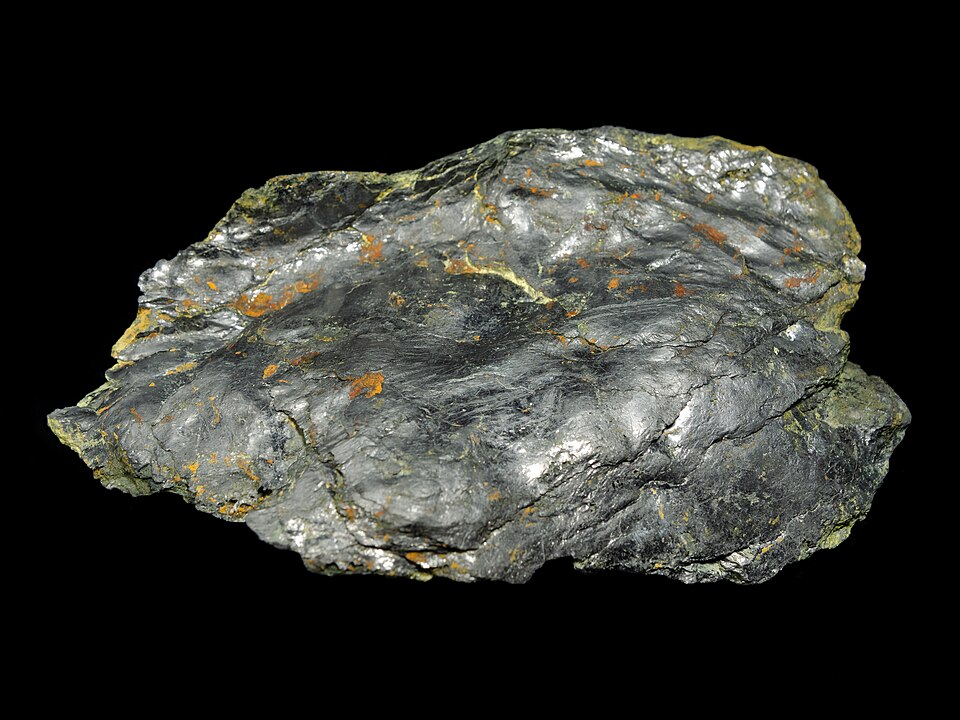
\includegraphics[width=0.36\linewidth]{images/book2/graphite.jpg}

{\small Spesimen grafit alam, dengan kilap logamnya. Foto: Zbynek
Burival, CC BY-SA 4.0.}
\end{omfigure}

\section{Kristal molekuler}

\begin{definition}[Kristal molekuler]\label{def:b1:crystals-ionic-covalent:molecular-crystal}
\emph{Kristal molekuler}\index{kristal molekuler} adalah \omterm{def:b1:crystals-metals:crystal}{kristal} yang
tersusun atas molekul-molekul yang diikat oleh gaya-gaya antarmolekul
--- \omterm{def:b1:intermolecular-forces-solvents:vdw}{interaksi van der Waals} dan, jika memungkinkan, \omterm{def:b1:intermolecular-forces-solvents:hbond}{ikatan hidrogen} ---
sementara setiap molekul mempertahankan ikatan-ikatan kovalennya
sendiri: diiodin, es kering \ce{CO2(s)}, es, gula.
\end{definition}

\begin{proposition}[Sifat-sifat kristal molekuler]\label{prop:b1:crystals-ionic-covalent:molecular}
\omterm{def:b1:crystals-ionic-covalent:molecular-crystal}{Kristal molekuler} lunak serta meleleh atau menyublim pada suhu rendah,
karena hanya gaya-gaya antarmolekul yang lemah yang diputus; \omterm{def:b1:crystals-metals:crystal}{kristal} ini
tidak menghantarkan listrik.
\end{proposition}
\admitted

\begin{example}[Es]\label{ex:b1:crystals-ionic-covalent:ice}
Dalam es biasa, setiap molekul air terikat dengan \omterm{def:b1:intermolecular-forces-solvents:hbond}{ikatan hidrogen} pada
empat molekul lain di sudut-sudut sebuah tetrahedron: dua melalui
hidrogennya sendiri dan dua melalui pasangan-pasangan elektron bebasnya.
Jejaring heksagonal yang terbuka ini, yang dipaksakan oleh arah \omterm{def:b1:intermolecular-forces-solvents:hbond}{ikatan
hidrogen}, menyisakan banyak ruang kosong: es kurang rapat daripada air
cair, yang jejaringnya sebagian terputus dan molekul-molekulnya saling
mendekat. Simetri heksagonal jejaring itu tampak pada bentuk \omterm{def:b1:crystals-metals:crystal}{kristal}
salju yang bersimetri enam.
\end{example}

\begin{omfigure}
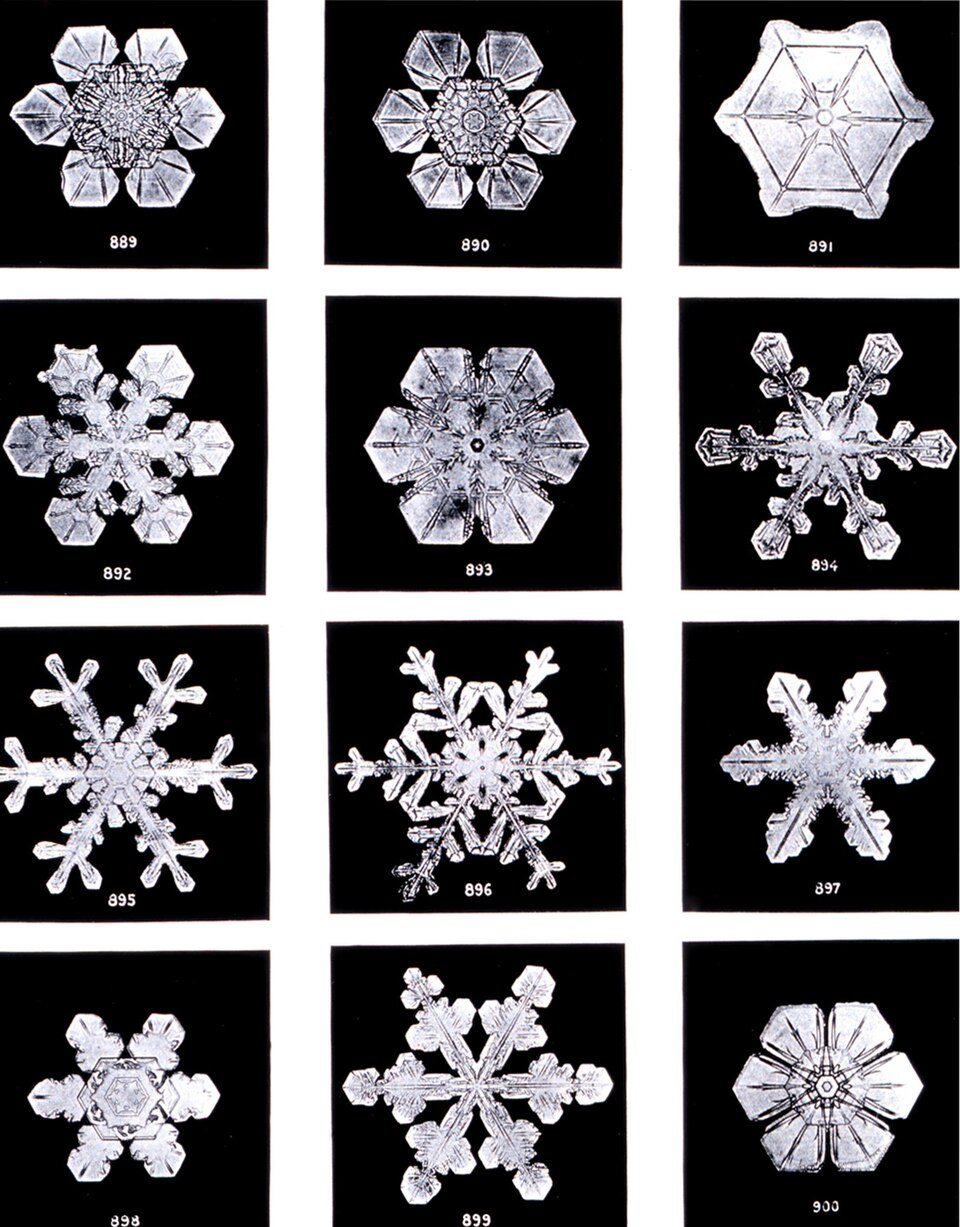
\includegraphics[width=0.38\linewidth]{images/book2/bentley-snowflakes.jpg}

{\small \omterm{def:b1:crystals-metals:crystal}{Kristal} salju yang dipotret Wilson Bentley sekitar tahun 1902:
setiap \omterm{def:b1:crystals-metals:crystal}{kristal} bersimetri enam, jejak jejaring heksagonal \omterm{def:b1:intermolecular-forces-solvents:hbond}{ikatan hidrogen}
dalam es. Domain publik.}
\end{omfigure}

\section{Membandingkan keempat jenis padatan}

\begin{center}
\small
\begin{tabular}{lllll}
\hline
padatan & partikel & kohesi & sifat & contoh \\
\hline
logam & kation, elektron & \omterm{def:b1:crystals-metals:metallic-bond}{ikatan logam} & konduktor, ulet & \ce{Cu}, \ce{Fe}, \ce{Na} \\
ion & kation, anion & elektrostatik & keras, rapuh, isolator & \ce{NaCl}, \ce{CaF2} \\
kovalen & atom & \omterm{def:b1:lewis-resonance-vsepr:lewis}{ikatan kovalen} & sangat keras, titik leleh tinggi & intan, \ce{SiO2} \\
molekuler & molekul & van der Waals, ikatan H & lunak, titik leleh rendah & \ce{I2}, es \\
\hline
\end{tabular}
\end{center}

\begin{remark}[Sebuah kesinambungan]\label{rem:b1:crystals-ionic-covalent:continuum}
Golongan-golongan itu adalah idealisasi. Seng sulfida mempunyai ikatan
yang sebagian ionik dan sebagian kovalen, itulah sebabnya jarak
sulfida--seng-nya lebih pendek daripada jumlah \omterm{def:b1:periodicity:radius}{jari-jari ionnya}; grafit
kovalen di dalam lapisannya dan molekuler di antara lapisan-lapisannya.
Selisih \omterm{def:b1:periodicity:electronegativity}{keelektronegatifan} (\cref{prop:b1:periodicity:en-trend}) menjadi
pedomannya: makin besar selisihnya, makin ionik padatannya.
\end{remark}

\section{Latihan}

\begin{exercise}[$\star$]\label{exo:b1:crystals-ionic-covalent:1}
Pada sel garam batu, hitunglah kation dan anionnya, tentukan koordinasi
masing-masing, dan periksalah bahwa rumus \ce{NaCl} terpenuhi.
\end{exercise}

\begin{exercise}[$\star$]\label{exo:b1:crystals-ionic-covalent:2}
Sesium klorida mempunyai $a = \qty{412.3}{pm}$. Hitunglah jarak \ce{Cs-Cl}
terpendek dan banyaknya satuan rumus per sel.
\end{exercise}

\begin{exercise}[$\star$]\label{exo:b1:crystals-ionic-covalent:3}
Dengan jari-jari $r(\ce{Na+}) = \qty{102}{pm}$ dan $r(\ce{Cl-}) =
\qty{181}{pm}$, hitunglah \omterm{def:b1:crystals-ionic-covalent:radius-ratio}{rasio jari-jari} \ce{NaCl} dan ramalkan
koordinasi kationnya.
\end{exercise}

\begin{exercise}[$\star$]\label{exo:b1:crystals-ionic-covalent:4}
Golongkan sebagai logam, ion, kovalen, atau molekuler: tembaga, natrium
klorida, intan, diiodin, kuarsa \ce{SiO2}, es, kalsium fluorida.
\end{exercise}

\begin{exercise}[$\star\star$]\label{exo:b1:crystals-ionic-covalent:5}
Buktikan bahwa struktur garam batu menuntut $r_+/r_- \ge \sqrt2 - 1$.
\end{exercise}

\begin{exercise}[$\star\star$]\label{exo:b1:crystals-ionic-covalent:6}
Hitunglah massa jenis natrium klorida dari $a = \qty{564.1}{pm}$
($M(\ce{NaCl}) = \qty{58.44}{g/mol}$), lalu bandingkan dengan
\qty{2.17}{g/cm^3}.
\end{exercise}

\begin{exercise}[$\star\star$]\label{exo:b1:crystals-ionic-covalent:7}
Hitunglah massa jenis sesium klorida ($M = \qty{168.36}{g/mol}$,
$a = \qty{412.3}{pm}$), lalu bandingkan dengan nilai terukur
\qty{3.99}{g/cm^3}.
% ledger: rho:CsCl
\end{exercise}

\begin{exercise}[$\star\star$]\label{exo:b1:crystals-ionic-covalent:8}
Untuk sfalerit ($a = \qty{540.9}{pm}$, $M = \qty{97.44}{g/mol}$),
hitunglah jarak \ce{Zn-S} dan massa jenisnya, lalu bandingkan dengan
nilai terukur \qty{4.04}{g/cm^3}.
% ledger: rho:ZnS
\end{exercise}

\begin{exercise}[$\star\star$]\label{exo:b1:crystals-ionic-covalent:9}
Grafit mempunyai sel heksagonal dengan $a = \qty{245.6}{pm}$ dan
$c = \qty{669.6}{pm}$, yang memuat 4 atom. Hitunglah jarak \ce{C-C} di
dalam satu lapisan ($a/\sqrt3$), jarak antarlapisan ($c/2$), dan massa
jenisnya. Mengapa grafit kurang rapat daripada intan?
\end{exercise}

\begin{exercise}[$\star\star\star$]\label{exo:b1:crystals-ionic-covalent:10}
Buktikan bahwa \omterm{def:b1:crystals-metals:compactness}{kekompakan} intan adalah $\pi\sqrt3/16$, lalu jelaskan
mengapa bahan yang paling keras justru termasuk yang paling tidak
kompak.
\end{exercise}

\begin{exercise}[$\star\star\star$]\label{exo:b1:crystals-ionic-covalent:11}
Silikon berstruktur intan dengan $a = \qty{543.1}{pm}$. Hitunglah
panjang ikatan \ce{Si-Si}, \omterm{def:b1:periodicity:radius}{jari-jari kovalen} silikon, dan massa jenisnya
($M = \qty{28.09}{g/mol}$); bandingkan dengan \qty{2.33}{g/cm^3}.
\end{exercise}

\begin{exercise}[$\star\star\star$]\label{exo:b1:crystals-ionic-covalent:12}
Rubidium klorida mempunyai $r(\ce{Rb+}) = \qty{152}{pm}$ (enam tetangga)
dan $r(\ce{Cl-}) = \qty{181}{pm}$. Struktur apakah yang diramalkan aturan
\omterm{def:b1:crystals-ionic-covalent:radius-ratio}{rasio jari-jari}? Pada kondisi biasa, zat ini bertipe garam batu dengan
$a = \qty{658.1}{pm}$: periksalah jarak \ce{Rb-Cl}, lalu kemukakan
mengapa aturan itu gagal di sini.
% ledger: rion:Rb+VI, rion:Cl-VI, lat:RbCl
\end{exercise}

\section{Soal: Fluorit, Mineral dan Lensa}

\begin{problem}[{Soal akhir pekan --- sel fluorit, \omterm{def:b1:crystals-ionic-covalent:radius-ratio}{rasio jari-jarinya},
dua kerabatnya (\ce{Li2O} dan intan), dan massa jenis fluorit yang
dihitung dari selnya}]
\label{pb:b1:crystals-ionic-covalent:1}
Fluorit, \ce{CaF2}, adalah sebuah mineral; jika ditumbuhkan sebagai \omterm{def:b1:crystals-metals:crystal}{kristal}
besar yang jernih, mineral ini menjadi lensa yang meneruskan cahaya
ultraungu. Selnya kubus, $a =
\qty{546.3}{pm}$; \ce{Ca^{2+}} pada \omterm{def:b1:crystals-metals:lattice}{kisi}
FCC, \ce{F-} di situs-situs tetrahedral. Jari-jari: $r(\ce{Ca^{2+}}) = \qty{112}{pm}$ (delapan tetangga), $r(\ce{F-}) = \qty{131}{pm}$ (empat
tetangga). Massa molar (g/mol): \ce{Ca} 40.08, \ce{F} 19.00, \ce{Li}
6.94, \ce{O} 16.00, \ce{C} 12.01, \ce{Si} 28.09;
$N_A = \qty{6.022e23}{mol^{-1}}$.
% ledger: lat:CaF2, rion:Ca2+VIII, rion:F-IV, aw:Ca, aw:F, aw:Li, aw:O,
% aw:C, aw:Si, const:NA

\medskip
\noindent\textbf{Bagian I --- Sel.}
\begin{enumerate}
  \item Tentukan posisi ion-ion \ce{Ca^{2+}} di dalam sel dan hitunglah
        banyaknya.
  \item Berapa banyak \omterm{def:b1:crystals-metals:site}{situs tetrahedral} di dalam sel itu? Turunkan
        banyaknya ion \ce{F-} dan periksalah rumusnya.
  \item Berapa koordinasi \ce{F-}? Koordinasi \ce{Ca^{2+}}?
  \item Hitunglah jarak \ce{Ca-F} terpendek.
  \item Bandingkan dengan jumlah \omterm{def:b1:periodicity:radius}{jari-jari ionnya}.
  \item Hitunglah jarak \ce{F-F} terpendek dan nyatakan apakah
        anion-anion itu bersentuhan.
\end{enumerate}

\medskip
\noindent\textbf{Bagian II --- \omterm{def:b1:crystals-ionic-covalent:radius-ratio}{Rasio jari-jari}.}
\begin{enumerate}[resume]
  \item Hitunglah $x = r_+/r_-$.
  \item Koordinasi kation berapakah yang diizinkan aturan \omterm{def:b1:crystals-ionic-covalent:radius-ratio}{rasio
        jari-jari}?
  \item Mengapa \ce{CaF2} tidak dapat mengambil struktur sesium klorida,
        padahal kationnya berkoordinasi 8?
  \item Paparkan fluorit sebagai susunan kubus sederhana \ce{F-} dengan
        \ce{Ca^{2+}} di pusat separuh kubus-kubus kecilnya.
  \item Hitunglah \omterm{def:b1:crystals-metals:compactness}{kekompakan} fluorit.
\end{enumerate}

\medskip
\noindent\textbf{Bagian III --- Dua kerabat.}
Litium oksida, \ce{Li2O}, berstruktur antifluorit dengan
$a = \qty{461.9}{pm}$; $r(\ce{Li+}) = \qty{59}{pm}$ (empat tetangga),
$r(\ce{O^{2-}}) =
\qty{142}{pm}$ (delapan tetangga). Intan:
$a = \qty{356.7}{pm}$.
% ledger: lat:Li2O, rion:Li+IV, rion:O2-VIII, rho:Li2O, lat:C-diamond
\begin{enumerate}[resume]
  \item Di manakah ion-ion \ce{O^{2-}} dan \ce{Li+} di dalam sel
        antifluorit?
  \item Hitunglah jarak \ce{Li-O}, lalu bandingkan dengan jumlah
        jari-jarinya.
  \item Hitunglah massa jenis \ce{Li2O}, lalu bandingkan dengan nilai
        terukur \qty{2.01}{g/cm^3}.
  \item Struktur ion manakah yang mempunyai susunan posisi yang sama
        dengan intan?
  \item Hitunglah panjang ikatan \ce{C-C} dan massa jenis intan.
  \item Mengapa intan jauh kurang kompak daripada fluorit, padahal
        atom-atomnya mengisi jenis posisi yang sama?
\end{enumerate}

\medskip
\noindent\textbf{Bagian IV --- Massa jenis fluorit.}
\begin{enumerate}[resume]
  \item Hitunglah massa molar \ce{CaF2}.
  \item Hitunglah massa satu sel.
  \item Hitunglah volume satu sel, dalam \unit{cm^3}.
  \item Apa pengaruh satu kekosongan pada satu situs \ce{F-} di setiap
        seratus sel terhadap massa jenisnya?
  \item Hitunglah massa jenis fluorit dari selnya, lalu bandingkan dengan
        nilai terukur \qty{3.18}{g/cm^3}.
\end{enumerate}
% ledger: rho:CaF2
\end{problem}
